%
% section 4.1.1
%
\subsection{Πρωτόκολλο TCP -- Δομή Πακέτου}

\begin{inthebox}
\textbf{Προσοχή:} Η αντίστοιχη ενότητα στο βιβλίο περιέχει διάφορα λάθη και ανακρίβειες, έχοντας ανακατέψει τις λειτουργίες των επιπέδων Μεταφοράς και Διαδικτύου. Σε αυτή την παράγραφο γράφουμε την πραγματικότητα, χρησιμοποιώντας το παράδειγμα του βιβλίου.\\
\end{inthebox}


\emph{Παράδειγμα Σχολικού Βιβλίου:} Έστω ότι θέλουμε να αποστείλουμε ένα μήνυμα μέσω ηλεκτρονικού ταχυδρομείου. Ο χρήστης θα γράψει το μήνυμα του στην αντίστοιχη εφαρμογή και θα συμπληρώσει την διεύθυνση ηλεκτρονικού ταχυδρομείου του παραλήπτη. Η διεύθυνση αυτή (μαζί με την αντίστοιχη του αποστολέα) αποτελούν μέρος της επικεφαλίδας που προστίθεται στο μήνυμα που δημιουργείται από το επίπεδο εφαρμογής.

Θυμηθείτε ότι το επίπεδο εφαρμογής, λειτουργεί με εντολές που είναι γενικά κατανοητές από τον άνθρωπο: τα προγράμματα σε αυτό το επίπεδο συνεννοούνται κατά βάση με εντολές στα αγγλικά που μπορούμε πολλές φορές να στείλουμε και χειροκίνητα. Για παράδειγμα μια συνομιλία με ένα διακομιστή ηλεκτρονικού ταχυδρομείου ξεκινά με το χαιρετισμό ``helo'' (ναι, είναι με ένα ``l'') ή ``ehlo''. Όλες αυτές οι εντολές και τα δεδομένα (κείμενο) του χρήστη πρέπει ωστόσο να μεταφερθούν μέσα από το επίπεδο μεταφοράς.

Το επίπεδο εφαρμογής δεν ενδιαφέρεται -- και δεν γνωρίζει -- τους περιορισμούς του φυσικού μέσου. Όσο αφορά ένα πρόγραμμα ταχυδρομείου, ο χρήστης μπορεί να γράψει και να στείλει όσο μεγάλο (ή μικρό) μήνυμα θέλει. Το πρόγραμμα επικοινωνεί απευθείας με το αντίστοιχο στην άλλη μεριά: οι λεπτομέρειες της πραγματικής επικοινωνίας κρύβονται στα παρακάτω επίπεδα.

Ας υποθέσουμε λοιπόν ότι ο χρήστης έγραψε ένα μήνυμα μεγέθους 6000 octets (ή bytes, αν το προτιμάτε). Το επίπεδο μεταφοράς θα πρέπει να τα μεταφέρει μέσω του TCP, αφού πρώτα γίνει μια αρχική σύνδεση και συνεννόηση με τον παραλήπτη (το TCP είναι πρωτόκολλο με σύνδεση). Με ποιο τρόπο και για ποιο λόγο θα αποφασίσει το TCP να δημιουργήσει τη δική του μονάδα δεδομένων (τα τμήματα, ή segments) με κάποιο συγκεκριμένο μέγεθος; Θα μπορούσε να στείλει όλο το μήνυμα σε ένα τμήμα;

Σύμφωνα με αυτά που ξέρουμε η απάντηση είναι ναι: Το TCP μπορεί να δημιουργήσει ένα τμήμα των 6000 bytes: τα τμήματα του TCP ενθυλακώνονται πάντα σε αυτοδύναμα πακέτα IP, και αυτά με τη σειρά τους ενθυλακώνονται στην αντίστοιχη μονάδα δεδομένων του κατώτερου επίπεδου (π.χ. σε πλαίσια Ethernet). Στο επίπεδο Διαδικτύου, τα πακέτα IP μπορούν να υποστούν κατάτμηση (fragmentation) αν το μέγεθος τους είναι τέτοιο που δεν μπορούν να ενθυλακωθούν σε πλαίσια. Θα μπορούσε λοιπόν το TCP να αφήσει αυτή τη λειτουργία στο IP. Υπάρχει λόγος να μην το κάνει;

Ναι. Όταν τα αυτοδύναμα πακέτα IP διασπώνται σε fragments, η απόδοση μειώνεται. Το κάθε fragment έχει δική του επικεφαλίδα και άρα μεταφέρει λιγότερα χρήσιμα δεδομένα από ότι ένα μη-διασπασμένο αυτοδύναμο πακέτο. Επίσης αν ένα fragment χαθεί ή καταστραφεί, είναι πλέον αδύνατο να συναρμολογηθεί το αντίστοιχο αυτοδύναμο πακέτο IP. Όμως αυτό το πακέτο έχει μέσα του πολλά δεδομένα (ένα ολόκληρο ``μεγάλου μεγέθους'' τμήμα): το επίπεδο μεταφοράς θα χρειαστεί να ξαναστείλει όλο το τμήμα. Θυμηθείτε ότι το IP είναι πρωτόκολλο τύπου ``best effort'': δεν παρέχει αξιοπιστία μετάδοσης και ούτε έχει κάποιο μηχανισμό να μεταδώσει ξανά fragment ή πακέτο IP που χάθηκε ή καταστράφηκε. Αυτό θα πρέπει να γίνει στο επίπεδο μεταφοράς.

Για να βελτιστοποιήσουμε την απόδοση, στην έναρξη της επικοινωνίας και οι δυο μεριές δηλώνουν το μέγιστο μέγεθος τμήματος που μπορούν να χρησιμοποιήσουν. Αυτό είναι γενικά γνωστό ως Maximum Segment Size (MSS). Δεν γίνεται κάποια διαπραγμάτευση μεταξύ των δύο άκρων: είναι απλά μια δήλωση. Σε γενικές γραμμές, επιλέγεται μια τιμή τέτοια ώστε να μη χρειαστεί να γίνει IP fragmentation: μια τέτοια τιμή προφανώς είναι κοντά στη μέγιστη μονάδα μεταφοράς του φυσικού μέσου (MTU), αφού ληφθούν υπόψη και οι επικεφαλίδες που θα προστεθούν σε κάθε επίπεδο. Σημειώστε ότι δεν θα χρησιμοποιηθεί αναγκαστικά η τιμή MSS για όλα τα τμήματα: απλά είναι η μέγιστη δυνατή. Η πραγματική μπορεί να είναι μικρότερη και ρυθμίζεται από παράγοντες όπως ο έλεγχος ροής (το πεδίο ``παράθυρο'').

Στο παράδειγμα μας, έστω ότι τελικά ανακαλύψαμε ότι μια κατάλληλη τιμή είναι τα 600 bytes. Τα αρχικά δεδομένα (6000 bytes) από το επίπεδο εφαρμογής θα γίνουν 10 τμήματα των 600 bytes στο επίπεδο μεταφοράς. Σε καθένα από αυτά τα 10 τμήματα θα προστεθεί (κατ'ελάχιστον) μια επικεφαλίδα 20 bytes για το TCP και μια ακόμα 20 bytes στο επίπεδο IP. Προφανώς το επίπεδο πρόσβασης δικτύου θα πρέπει να μπορεί να δημιουργήσει πλαίσια με μήκος δεδομένων τουλάχιστον 640 bytes.

\begin{figure}[!ht]
 \centering
 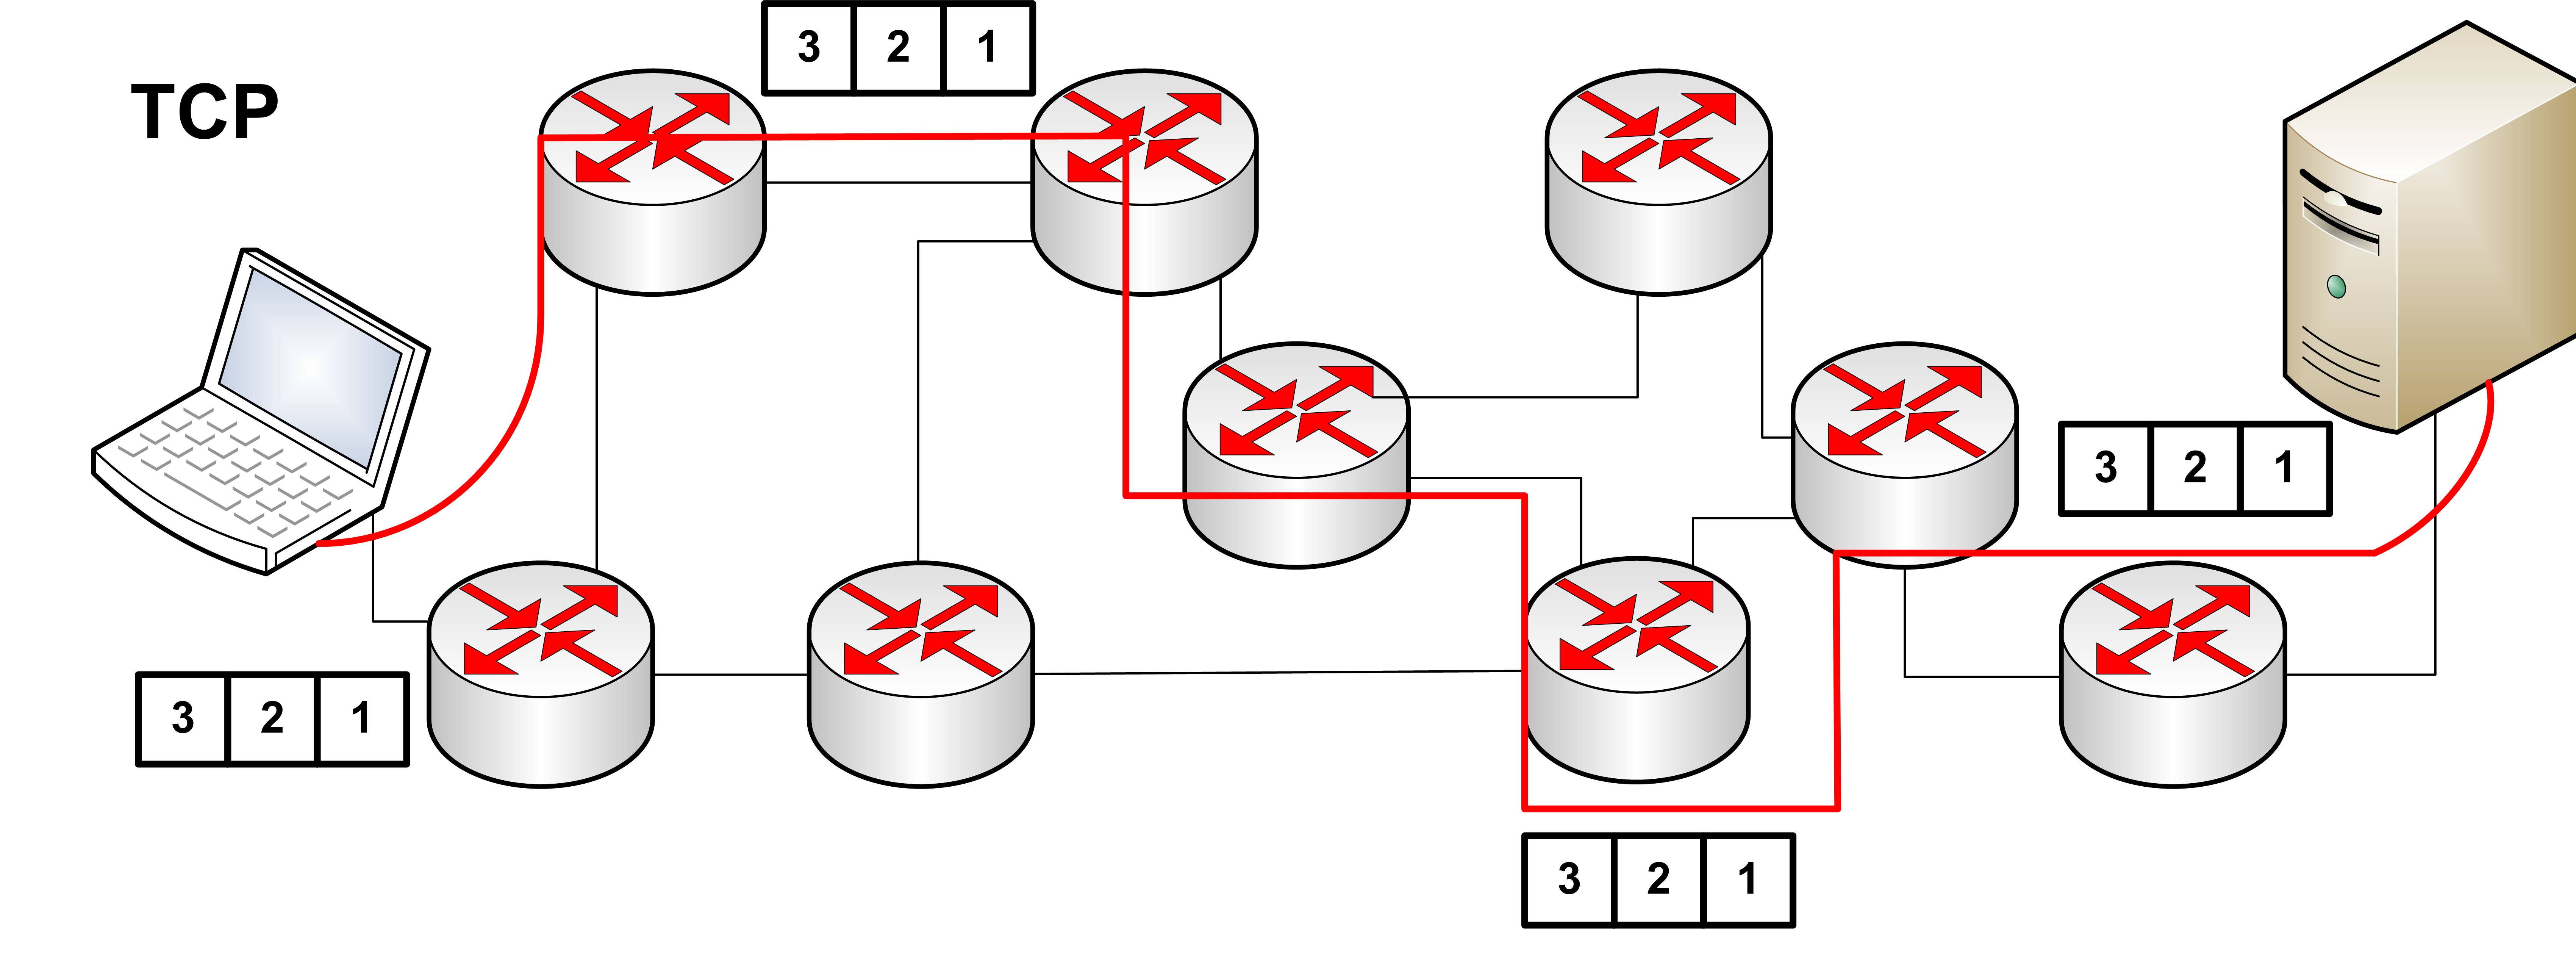
\includegraphics[width=0.85\textwidth]{images/chapter4/4-1-w}
 \caption {\textsl{Επικοινωνία TCP - ΛΑΘΟΣ}}
 \label{4-1-w}
\end{figure}

\begin{figure}[!ht]
 \centering
 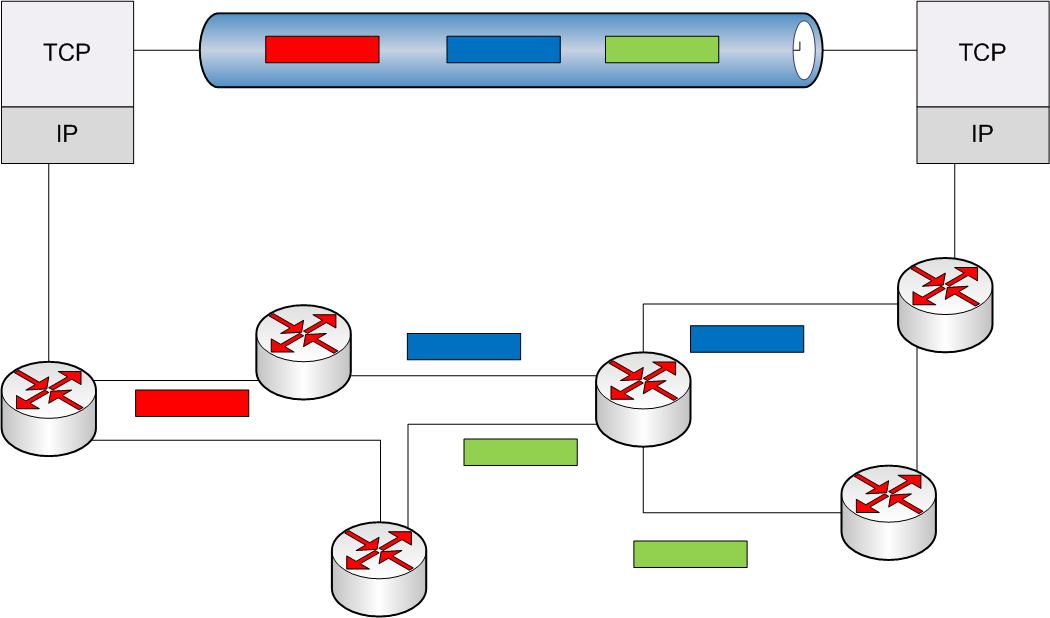
\includegraphics[width=0.85\textwidth]{images/chapter4/4-1-r}
 \caption {\textsl{Επικοινωνία TCP - ΣΩΣΤΗ}}
 \label{4-1-r}
\end{figure}

Η εικόνα \ref{4-1-w} στο βιβλίο σας είναι επίσης λάθος: ο συγγραφέας προσπαθεί να δείξει ότι υπάρχει ένα νοητό κύκλωμα στο TCP αλλά φτιάχνει μια συγκεκριμένη διαδρομή μέσα από δρομολογητές: οι δρομολογητές όμως δεν ασχολούνται με το επίπεδο μεταφοράς αλλά με το επίπεδο διαδικτύου. Όπως γνωρίζουμε το κάθε αυτοδύναμο IP πακέτο αντιμετωπίζεται χωριστά από τους δρομολογητές και πακέτα της ίδιας μετάδοσης μπορεί τελικά να ακολουθήσουν διαφορετικές διαδρομές μέσα από το επικοινωνιακό υποδίκτυο. Η γραμμή που ενώνει εδώ τους κόμβους μέσα από μια συγκεκριμένη διαδρομή είναι άκυρη. Για ένα σωστό σχήμα δείτε την εικόνα \ref{4-1-r} όπου φαίνεται καθαρά ότι όσο αφορά το TCP η επικοινωνία είναι μια ευθεία γραμμή (end to end) αλλά στην πραγματικότητα τα αυτοδύναμα πακέτα μπορεί να κινούνται από διαφορετικές διαδρομές.

Όταν τα τμήματα φτάσουν στο άλλο άκρο θα επανασυνδεθούν για να σχηματίσουν το αρχικό μήνυμα των 6000 οκτάδων. Καθώς στην πραγματικότητα τα τμήματα μεταφέρονται μέσω ενθυλάκωσης σε αυτοδύναμα πακέτα IP, είναι πιθανόν να φτάσουν με διαφορετική σειρά (κάθε IP πακέτο μπορεί να ακολουθήσει διαφορετική διαδρομή). Επίσης στην διαδρομή ενδεχομένως κάποια πακέτα IP να καταστραφούν: το πρωτόκολλο IP δεν παρέχει λειτουργίες αξιόπιστης μετάδοσης. Τα τμήματα που μεταφέρονται σε προβληματικά (ή χαμένα) πακέτα IP θα πρέπει να μεταδοθούν ξανά.

Ένα ακόμα πρόβλημα που προκύπτει και πρέπει να λυθεί από το πρωτόκολλο TCP, είναι ο διαχωρισμός των δεδομένων της κάθε σύνδεσης: ανά πάσα στιγμή ένας υπολογιστής -- πελάτης μπορεί να είναι συνδεδεμένος με πολλαπλές συνδέσεις σε ένα εξυπηρετητή. Φανταστείτε για παράδειγμα ότι με τον υπολογιστή σας βλέπετε μια ιστοσελίδα από ένα εξυπηρετητή. Κάνετε κλικ σε ένα σύνδεσμο και αρχίζετε να κατεβάζετε κάποιο αρχείο από την ίδια ιστοσελίδα. Πως γνωρίζει ο φυλλομετρητής σας ποια δεδομένα ανήκουν στην ιστοσελίδα και ποια στο αρχείο που κατεβάζετε, αφού μάλιστα είναι από τον ίδιο εξυπηρετητή.

Σημειώστε ότι αυτό το πρόβλημα δεν υπάρχει όταν αναφερόμαστε σε διαφορετικούς εξυπηρετητές: εκεί είναι δυνατόν να γίνει ο διαχωρισμός ήδη από το πρωτόκολλο δικτύου με βάση τη διεύθυνση IP. Ας δούμε τώρα το ίδιο πρόβλημα από τη μεριά του εξυπηρετητή: είναι δυνατόν (και συμβαίνει συχνά) το ίδιο μηχάνημα να παρέχει πολλές υπηρεσίες. Π.χ. σε μια μικρή εταιρεία δεν είναι σπάνιο ένας εξυπηρετητής να διαθέτει ταυτόχρονα υπηρεσία ηλεκτρονικού ταχυδρομείου (email), ιστοσελίδων (web), μεταφοράς αρχείων (ftp) κ.α. Πως ο εξυπηρετητής διαχωρίζει ποια τμήματα TCP αναφέρονται σε κάθε υπηρεσία;

Όσο αφορά το TCP υπάρχει ένα είδος \emph{πολυπλεξίας} δίνεται δηλ. η δυνατότητα πολλές διεργασίες μέσα στον ίδιο τερματικό κόμβο (host) να χρησιμοποιούν τις υπηρεσίες του πρωτοκόλλου \emph{ταυτόχρονα}. Η δυνατότητα αυτή εξασφαλίζεται με τα πεδία \emph{Θύρας Προέλευσης} και \emph{Θύρας Προορισμού}. Όπως ακριβώς το πρωτόκολλο IP μας πηγαίνει μέχρι ένα συγκεκριμένο μηχάνημα χρησιμοποιώντας τη διεύθυνση IP, οι θύρες μας οδηγούν σε μια συγκεκριμένη εφαρμογή πελάτη ή εξυπηρετητή (συγκεκριμένη σύνδεση) όταν έχουμε πλέον φτάσει στον προορισμό μας.

Στη φάση της επανασύνθεσης του αρχικού μηνύματος, το TCP πρέπει να γνωρίζει ποια είναι η προέλευση (source) και ποιος ο προορισμός (destination) του μηνύματος. Το TCP εξασφαλίζει την \emph{αξιοπιστία} της σύνδεσης με:

\begin{itemize}
\item Την εγκατάσταση νοητής σύνδεσης από την προέλευση στο προορισμό.
\item Τον τεμαχισμό των δεδομένων σε τμήματα κατάλληλα για το δίκτυο.
\item Την επιβεβαίωση στην παραλαβή των δεδομένων.
\item Την τοποθέτηση των τμημάτων στη σωστή σειρά κατά την παραλαβή (και την επαναμετάδοση τμημάτων που χάθηκαν ή καταστράφηκαν).
\end{itemize}

\begin{figure}[!ht]
 \centering
 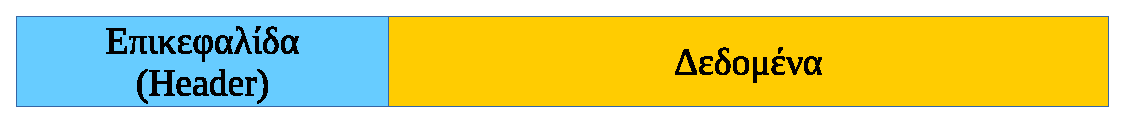
\includegraphics[width=0.85\textwidth]{images/chapter4/4-2}
 \caption {\textsl{Τμήμα TCP}}
 \label{4-2}
\end{figure}

Όλες οι πληροφορίες που είναι απαραίτητες για τον έλεγχο και την ανασύνθεση του αρχικού μηνύματος περιέχονται στην \emph{επικεφαλίδα (header)} που δημιουργείται στο σχηματισμό του τμήματος. Η επικεφαλίδα είναι μια σειρά από οκτάδες που προστίθενται στην αρχή του τμήματος, πριν από τα πραγματικά δεδομένα (σχήμα \ref{4-2}).

Το ελάχιστο μέγεθος της επικεφαλίδας είναι 20 οκτάδες και το μέγιστο 60, αν υπάρχει το προαιρετικό τμήμα. Στο σχήμα \ref{4-3} βλέπουμε τα πεδία της επικεφαλίδας του TCP που εξετάζουμε παρακάτω.

\begin{figure}[!ht]
 \centering
 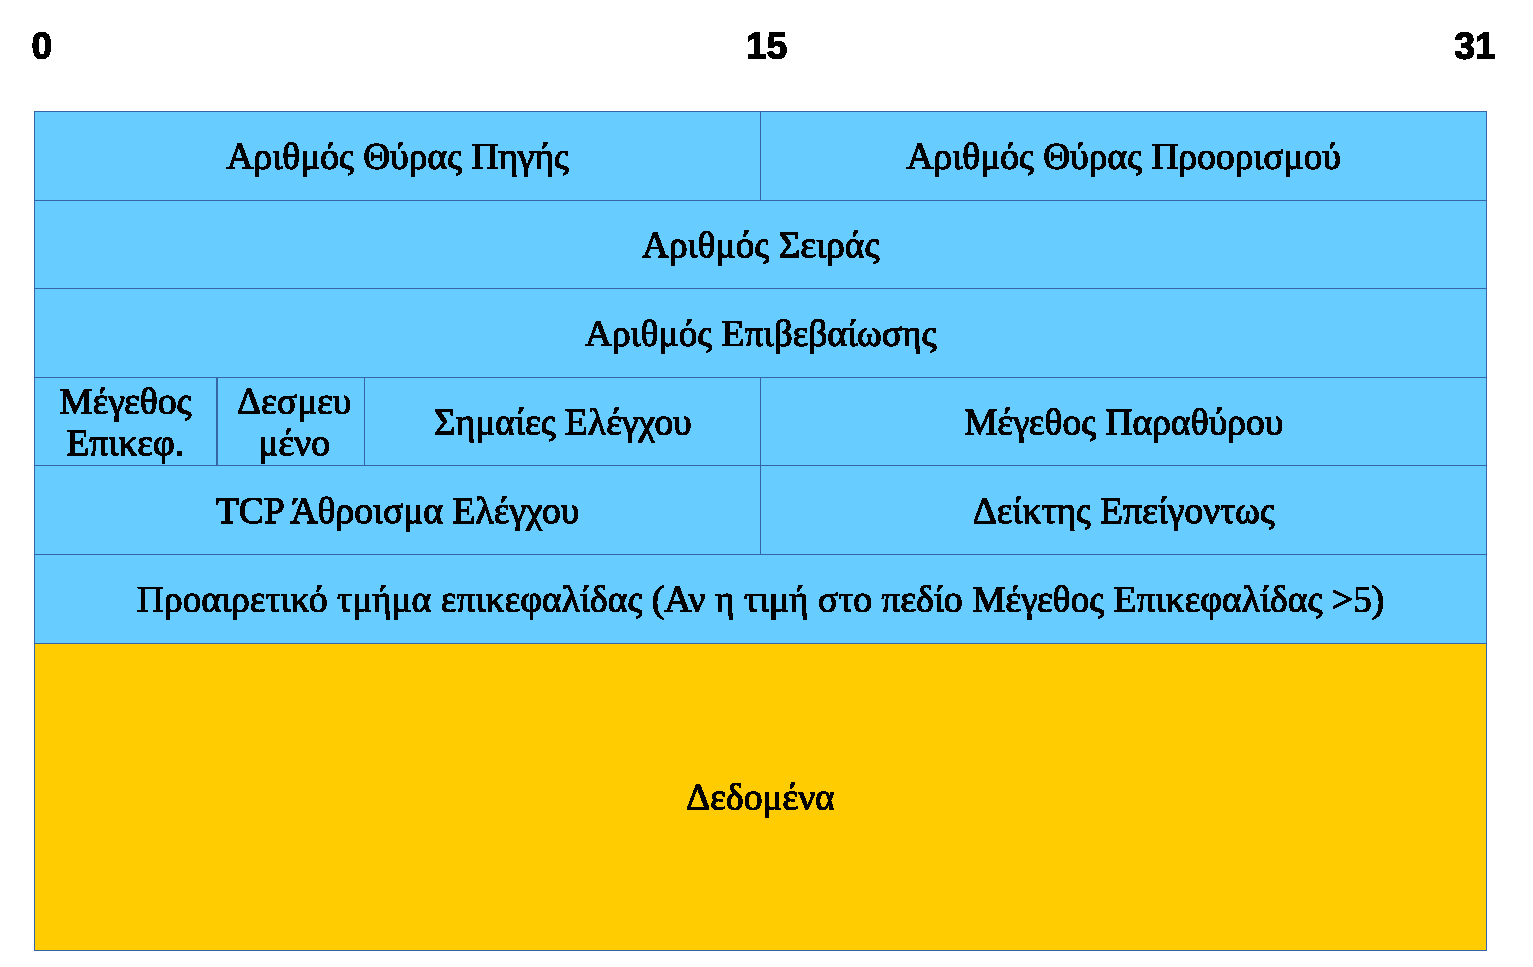
\includegraphics[width=0.95\textwidth]{images/chapter4/4-3}
 \caption {\textsl{Πεδία Επικεφαλίδας TCP Τμήματος}}
 \label{4-3}
\end{figure}

\begin{itemize}
\item \textbf{Αριθμός Θύρας Προέλευσης (Source Port number) και Αριθμός Θύρας Προορισμού (Destination Port Number):} Όπως αναφέραμε προηγουμένως, οι δύο αυτοί αριθμοί χρησιμεύουν στην ταυτοποίηση διαφορετικών συνομιλιών TCP. Για παράδειγμα ένα πρόγραμμα εξυπηρέτησης ηλεκτρονικού ταχυδρομείου χρησιμοποιεί (βάση προτύπου) τη θύρα TCP 25, ενώ ένα αντίστοιχο ιστοσελίδων τη θύρα 80. Αν οι δύο αυτές υπηρεσίες εκτελούνται στο ίδιο μηχάνημα, όλα τα τμήματα που λαμβάνονται με θύρα προορισμού 25 προωθούνται στο ηλεκτρονικό ταχυδρομείο ενώ αυτά με θύρα προορισμού 80 στο πρόγραμμα εξυπηρέτησης ιστοσελίδων. Αν ο ίδιος πελάτης (από την ίδια διεύθυνση IP) συνδεθεί ταυτόχρονα και στις δύο υπηρεσίες, τα τμήματα θα έχουν επίσης και διαφορετικές θύρες αποστολέα: έτσι και τα τμήματα -- απαντήσεις από τον εξυπηρετητή θα μπορούν αντίστοιχα να διαχωριστούν στις αντίστοιχες εφαρμογές στον πελάτη. \emph{Το παράδειγμα στο βιβλίο σας είναι λάθος:} Αν οι συνδέσεις προέρχονται από διαφορετικούς υπολογιστές δεν μπορούμε να τα ξεχωρίσουμε με βάση τη θύρα αποστολέα. Οι θύρες αποστολέα επιλέγονται τυχαία στους πελάτες και μπορεί διαφορετικά μηχανήματα να χρησιμοποιούν την ίδια θύρα αποστολέα. Όμως ο διαχωρισμός γίνεται πλέον μέσω της διεύθυνσης IP στο επίπεδο δικτύου. Όταν το πρόγραμμα εξυπηρέτησης απαντά σε ένα πελάτη, προφανώς τα πεδία των θυρών αντιστρέφονται μεταξύ τους (η θύρα προέλευσης γίνεται αποστολής και η αποστολής προέλευσης). Τα πεδία αυτά έχουν μέγεθος 16 bit το καθένα, επιτρέποντας ένα μέγιστο 2\textsuperscript{16}=65536 θυρών.
\item \textbf{Αριθμός Σειράς (Sequence Number):} Ο αριθμός αυτός χρησιμεύει ώστε ο παραλήπτης να τοποθετεί τα τμήματα στη σωστή σειρά καθώς ανασυνθέτει τα αρχικά δεδομένα. Τα τμήματα μπορεί να έχουν παραληφθεί με διαφορετική σειρά από τη σειρά αποστολής καθώς ταξιδεύουν μέσα στο δίκτυο ενθυλακωμένα σε αυτοδύναμα πακέτα IP. Το TCP αριθμεί τα τμήματα με βάση τα octets, έτσι αν κάθε τμήμα αποτελείται από 600 octets, το πρώτο έχει αριθμό σειράς 0, το δεύτερο 600, το τρίτο 1200 κλπ (Σημείωση: πρόκειται για μια απλούστευση του σχολικού βιβλίου, τα πράγματα δεν είναι ακριβώς έτσι). Το πεδίο αυτό έχει μέγεθος 32 bit.
\item \textbf{Αριθμός Επιβεβαίωσης (Acknowledgement):} Ο αριθμός αυτός χρησιμοποιείται για να εξασφαλιστεί ότι κάθε τμήμα έχει φτάσει στον προορισμό του. Όταν ο παραλήπτης στο άλλο άκρο παραλάβει το τμήμα, στέλνει ένα νέο τμήμα επιβεβαίωσης (ACK) με συμπληρωμένο το πεδίο αυτό. Π.χ. ένα τμήμα επιβεβαίωσης με αριθμό επιβεβαίωσης 1201 σημαίνει ότι έχουν φτάσει όλα τα δεδομένα μέχρι και την οκτάδα 1200. Αν ο αποστολέας δεν παραλάβει τμήμα επιβεβαίωσης μέσα σε ένα συγκεκριμένο χρονικό διάστημα, θεωρεί ότι το τμήμα έχει χαθεί και μεταδίδεται ξανά. Το πεδίο αυτό έχει μέγεθος 32 bit, όπως και ο αριθμός σειράς.
\item \textbf{Μέγεθος Παραθύρου (Window):} Για να επιταχυνθεί η επικοινωνία το TCP δεν περιμένει παραλαβή της επιβεβαίωσης για να στείλει το επόμενο τμήμα. Όμως δεν είναι δυνατόν να αποστέλλονται συνεχώς δεδομένα γιατί ένας γρήγορος αποστολέας στο ένα άκρο μπορεί να ξεπεράσει την ταχύτητα με την οποία μπορεί να δεχθεί δεδομένα ένας πιο αργός παραλήπτης. Στο πεδίο Window το κάθε άκρο δηλώνει πόσα νέα δεδομένα μπορεί να απορροφήσει κάθε φορά, θέτοντας σε αυτό την τιμή των ελεύθερων οκτάδων του ενταμιευτή του (Ο ενταμιευτής ή buffer είναι ο προσωρινός χώρος όπου αποθηκεύονται τα τμήματα προκειμένου να επανασυνδεθούν και να προωθηθούν στο παραπάνω επίπεδο). Ένας παραλήπτης μπορεί να λαμβάνει δεδομένα πιο γρήγορα από ότι μπορεί να τα επεξεργαστεί με αποτέλεσμα ο διαθέσιμος χώρος στον ενταμιευτή να μειώνεται συνέχεια. Αν ο χώρος αυτός γεμίσει ο αποστολέας πρέπει προσωρινά να σταματήσει την αποστολή νέων δεδομένων διαφορετικά αυτά θα απορριφθούν. Ο παραλήπτης δηλώνει με το πεδίο Window ότι είναι έτοιμος να δεχτεί νέα δεδομένα. Το πεδίο αυτό έχει μέγεθος 16 bit.
\item \textbf{Άθροισμα Ελέγχου (TCP Checksum):} Το πεδίο αυτό περιέχει ένα άθροισμα ελέγχου όλων των οκτάδων του τμήματος (επικεφαλίδας και δεδομένων). Στον υπολογισμό του αθροίσματος ελέγχου θεωρείται ότι το συγκεκριμένο πεδίο έχει τιμή μηδέν. Ο παραλήπτης στο άλλο άκρο υπολογίζει ξανά το άθροισμα από την αρχή και το συγκρίνει με αυτό που παρέλαβε. Αν τα δυο αποτελέσματα δεν είναι ίδια, το τμήμα θεωρείται κατεστραμμένο και απορρίπτεται. Το πεδίο αυτό έχει μέγεθος 16 bit.
\item \textbf{Μέγεθος Επικεφαλίδας (Data Offset):} Το πεδίο αυτό καθορίζει το μέγεθος της επικεφαλίδας σε λέξεις των 32bit. Για παράδειγμα αν η τιμή του πεδίου αυτού είναι 5, η επικεφαλίδα είναι 5Χ32 bit = 160 bit ή 20 bytes. (Μπορείτε απλά να πολλαπλασιάσετε αυτή τη τιμή με το 4 για να πάρετε τα bytes της επικεφαλίδας). Αν η επικεφαλίδα είναι μεγαλύτερη από 20 bytes (τιμή πεδίου μεγαλύτερη από 5) θα υπάρχουν επιπλέον επιλογές TCP στο \emph{Προαιρετικό τμήμα επικεφαλίδας}. Αν τα δεδομένα του προαιρετικού τμήματος δεν είναι πολλαπλάσια των 32bit (ώστε να συμπληρώνουν όλη τη γραμμή της επικεφαλίδας), συμπληρώνονται με μηδενικά στο τέλος (padding). Το πεδίο ``Μέγεθος Επικεφαλίδας'' έχει μέγεθος 4 bit.
\item \textbf{Οι σημαίες ελέγχου (flags)} είναι εννέα πεδία του ενός bit το καθένα και σηματοδοτούν διάφορες καταστάσεις που αφορούν το χειρισμό των συνδέσεων.  Τα σημαντικότερα από αυτά είναι:
\begin{enumerate}
\item \textbf{URG, Urgent Pointer, Δείκτης Επείγοντος:} Το πεδίο αυτό χρησιμοποιείται για να πληροφορήσει το άλλο άκρο για κάτι σημαντικό, π.χ. να προχωρήσει επειγόντως στην επεξεργασία της συγκεκριμένης οκτάδας. Αυτό μπορεί να συμβαίνει π.χ. αν ο χρήστης ζητήσει τη διακοπής της επικοινωνίας στέλνοντας ένα χαρακτήρα ελέγχου (π.χ. πιέζοντας CTRL+C (διακοπή) σε μια μεταφορά αρχείου μέσω FTP σε ένα σύστημα UNIX).
\item \textbf{ACK, Acknowledgement, Επιβεβαίωση:} Όταν τίθεται τιμή 1 σε αυτό το πεδίο, σημαίνει ότι το συγκεκριμένο τμήμα περιέχει επιβεβαίωση δεδομένων. Ο παραλήπτης του τμήματος θα πρέπει να εξετάσει το πεδίο ``Αριθμός Επιβεβαίωσης''.
\item \textbf{PSH, Push, Προώθηση:} Το πεδίο αυτό ενημερώνει τον παραλήπτη ότι πρέπει να προωθήσει όσο το δυνατόν πιο γρήγορα τα περιεχόμενα του τμήματος στο επίπεδο εφαρμογής. 
\item \textbf{RST, Reset, Επανεκκίνηση:} Το πεδίο αυτό επισημαίνει επανεκκίνηση / καθαρισμό της σύνδεσης.
\item \textbf{SYN, Syncrhonize, Συγχρονισμός:} Το πεδίο αυτό χρησιμεύει (μαζί με τον αριθμό σειράς) για το συγχρονισμό της εγκατάστασης μιας νέας σύνδεσης.
\item \textbf{FIN, Finalize, Ολοκλήρωση:} Το πεδίο αυτό ενημερώνει ότι ο αποστολέας έχει ολοκληρώσει την αποστολή δεδομένων.
\end{enumerate}
\end{itemize}

Η δομή του τμήματος TCP περιέχει όλες τις πληροφορίες που απαιτούνται για την παροχή επικοινωνίας με σύνδεση:

\begin{itemize}
\item \emph{Την εγκατάσταση σύνδεσης} με συμφωνημένες προδιαγραφές επικοινωνίας μεταξύ των δύο άκρων.
\item \emph{Την αξιοπιστία} στη μετάδοση δεδομένων. Όποια τμήματα χαθούν ή καταστραφούν θα μεταδοθούν ξανά.
\item \emph{Τον έλεγχο ροής δεδομένων} που επιτυγχάνεται με το πεδίο Window και έχει σκοπό να μην υπερφορτωθεί ένας αργός παραλήπτης από ένα γρήγορο αποστολέα.
\item \emph{Τον έλεγχο συμφόρησης δεδομένων:} που εξασφαλίζει ότι ένα αργό κανάλι επικοινωνίας δεν θα πλημμυρίσει με δεδομένα με κίνδυνο κατάρρευσης.
\end{itemize} 